\documentclass[problems]{esg8012pset} 
  \usepackage{amsmath}
  \usepackage{amssymb}
  \usepackage{enumerate}
  \usepackage{graphicx}
  \usepackage{hyperref}
  %\usepackage{siunitx}
  \providecommand{\uvec}[1]{{\hat{\bf{#1}}}}
  \usepackage{pgf,tikz}
  \usetikzlibrary{arrows}
  \makeatletter
  \newcommand{\interitemtext}[1]{%
    \begin{list}{}
     {\itemindent=0mm\labelsep=0mm
     \labelwidth=0mm\leftmargin=0mm
     \addtolength{\leftmargin}{-\@totalleftmargin}}
      \item #1
    \end{list}
  }
  \makeatother
  \renewcommand{\d}{\,d}
  \providecommand{\norm}[1]{\lVert#1\rVert}
\classname{Physics 8.012} 
\semester{Fall 2010} 
\problemsetnumber{7} 
\date{October 22} 
\duedate{Monday, November 1} 
\readingassignment{Kleppner and Kolenkow, \emph {An Introduction to Mechanics}, Chapter Four} 
\begin{document}
\section{Problem \thesection: K\&K 4.21}
  An unknown rope of linear mass density $\lambda$ (mass per unit length), is coiled on a smooth horizontal table. On end is pulled straight up with constant speed $v_0$.
  \begin{center}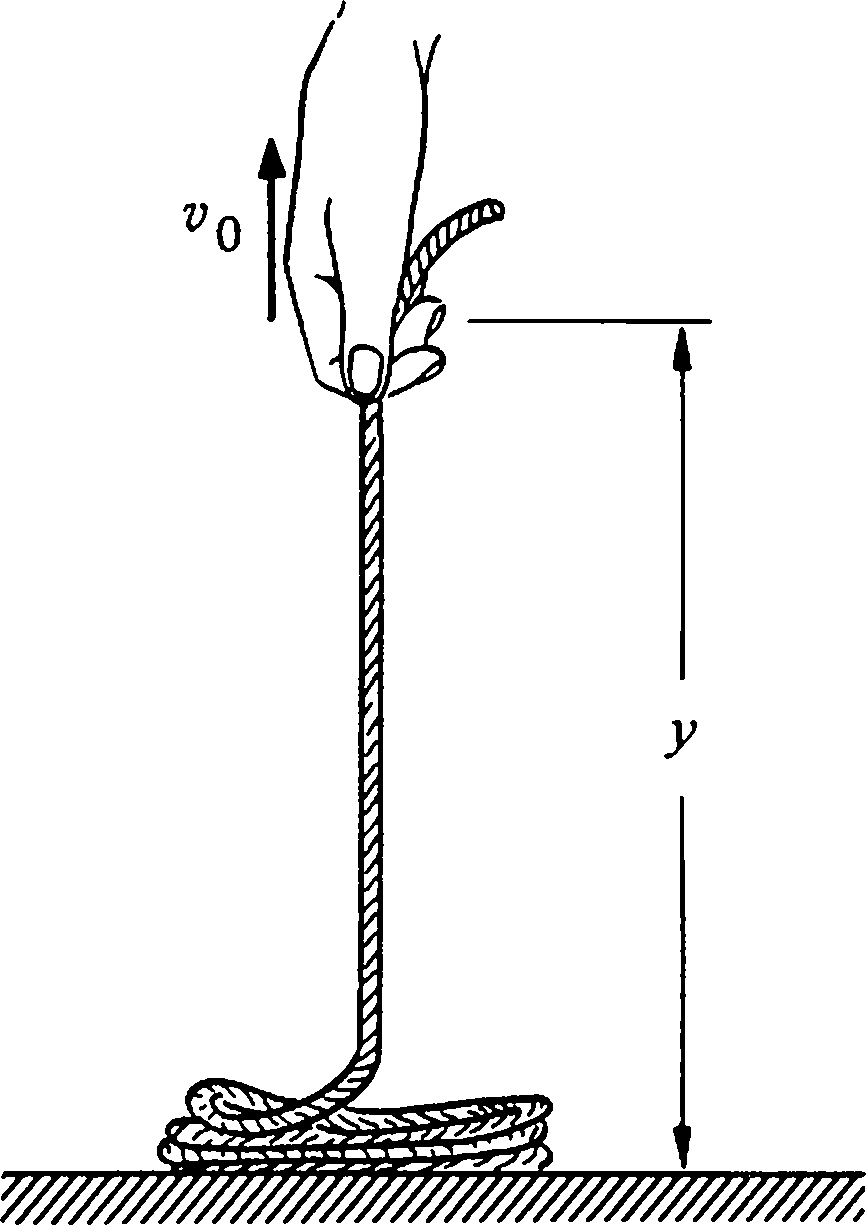
\includegraphics[width=0.2\textwidth]{ps07_1}\end{center}
  \begin{enumerate}[(a)]
  \item Find the force exerted on the end of the rope as a function of the height $y$ of the rope above the table.
    \item Compare the power delivered to the rope with the rate of change of the rope's total mechanical energy. Explain whether they should or should not be equal. Remember that the rope is not a rigid body.
  \end{enumerate}
\section{Problem \thesection: K\&K 4.23}
  Two superballs are dropped from a height above the ground. The ball on top has a mass $m_1$. The ball on the bottom has a mass $m_2$. Assume that the lower ball collides elastically with the ground. Then as the lower ball starts to move upward, it collides elastically with the upper ball that is still moving downwards. How high will the upper ball rebound in the air? Assume that $m_2 \gg m_1$. Hint: consider this collision from an inertial reference frame that moves upward with the same speed as the lower ball has after it collides with ground. What speed does the upper ball have in this reference frame after it collides with the lower ball?
  \begin{center}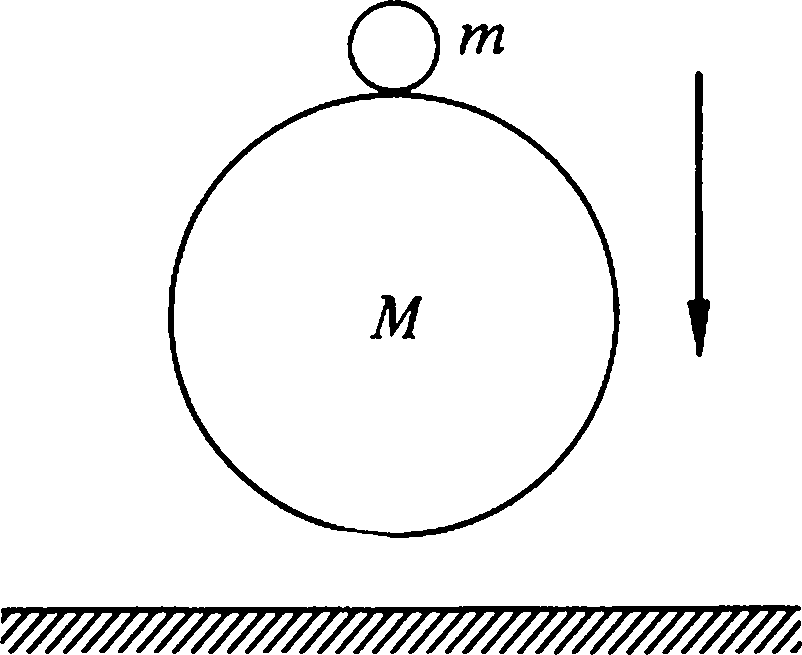
\includegraphics[width=0.25\textwidth]{ps07_2}\end{center}
\section{Problem \thesection: K\&K 4.25: (Elastic collision in two dimensions)}
  A proton makes a head-on collision with an unknown particle at rest. The proton rebounds straight back with $4 / 9$ of its initial kinetic energy. Find the ratio of the mass of the unknown particle to the mass of the proton, assuming that the collision is elastic.
\section{Problem \thesection: K\&K 4.27}
  A particle $A$ of mass $m$ is initially moving in the positive $x$-direction with a speed $v_{A,0}$ and collides elastically with a second particle $B$ of mass $2m$, which is initially at rest.  After the collision the particle $A$ moves with an unknown speed $v_{A,f}$, at an unknown angle $\theta_{A, f}$ with respect to the positive $x$-direction. After the collision, particle $B$ moves with an unknown speed $v_{B, f}$, at an angle $\theta_{2,f} = 45^{\circ}$ with respect to the positive $x$-direction.  Find $\theta_{A, f}$.
  \begin{center}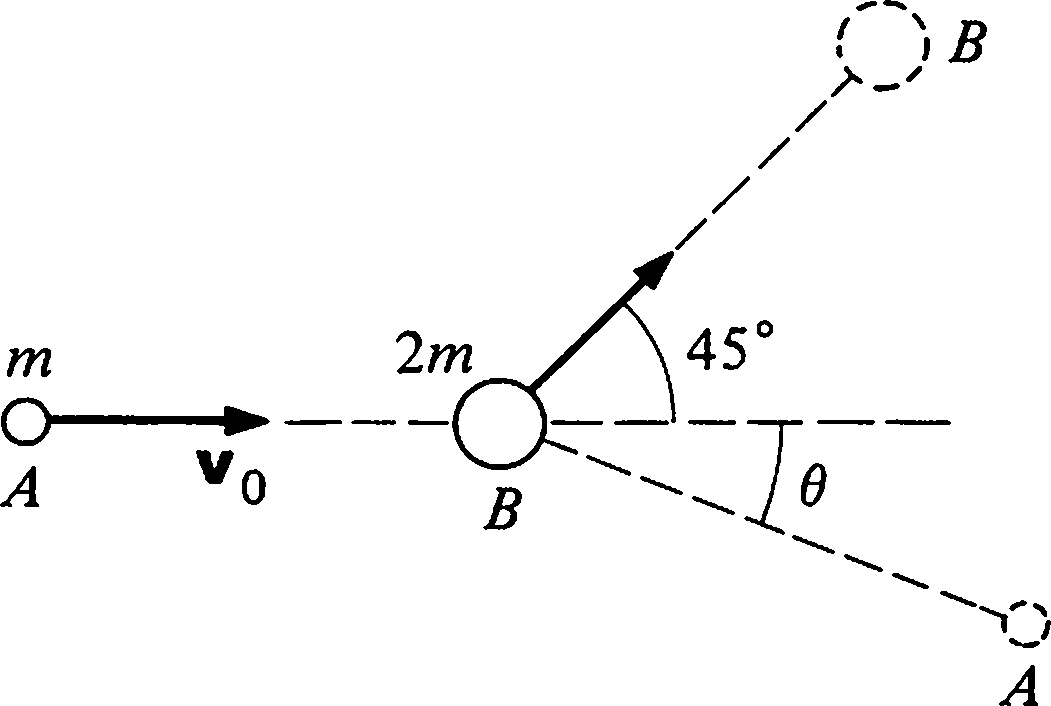
\includegraphics[width=0.3\textwidth]{ps07_3}\end{center}
\section{Problem \thesection: K\&K 4.28}
  A thin target of lithium is bombarded by helium nuclei of energy $E_0$. The lithium nuclei are initially at rest in the target but are essentially unbound. When a helium nucleus enters a lithium nucleus, a nuclear reaction can occur in which the compound nucleus splits apart into a boron nucleus and a neutron. The collision is inelastic, and the final kinetic energy is less than $E_0$ by 2.8 MeV. ($1\text{ MeV} = 10^6\text{ eV} = 1.6 \times 10^{-13}\text{ J}$). The relative masses of the particles are: helium, mass 4; lithium, mass 7; boron mass 10; neutron, mass 1. The reaction can be symbolized
  $${}^7\text{Li} + {}^4\text{He} \to {}^{10}\text{B} + {}^1\text{n} - 2.8\text{ MeV}.$$
  \begin{enumerate}[(a)]
  \item The minimum initial kinetic energy necessary for the reaction to take place is called the threshold energy, $E_{0,\text{threshold}}$. What is $E_{0,\text{threshold}}$ for which neutrons can be produced? What is the energy of the neutrons at this threshold?
    \item Show that if the incident kinetic energy falls in the range $$E_{0,\text{threshold}} < E_0 < E_{0,\text{threshold}} + 0.27\text{ MeV},$$ the neutrons ejected in the same direction as the incoming helium (forward direction) do not all have the same energy but must have one or the other of two possible energies. By considering the reaction in a reference frame moving with the velocity of the center of mass of the system, explain why there must be two distinct energies.
  \end{enumerate}
\section{Problem \thesection: K\&K 4.30}
  A particle of mass $m_1$ and velocity $\vec v_{1,0}$ by a particle of mass $m_2$ at rest in the laboratory frame is scattered elastically through a scattering angle $\theta$ in the center of mass frame.
  \begin{enumerate}[(a)]
    \item Find the final velocity of the incoming particle in the laboratory reference frame.
    \item Find the fractional loss of kinetic energy of the incoming particle. Is this the same in every reference frame? Explain.
  \end{enumerate}
\end{document}
